
\section{Introduction to On-Chain Governance} \label{sec:governance-intro}

Cardano is advancing towards a decentralized governance model designed to empower community participation and ensure robust decision-making processes. This model is detailed in CIP-1694, which outlines a framework for governance through a tricameral model and a structured decision-making process via seven different types of governance actions. A governance action is a transaction-triggered on-chain event with a time-limited window for execution.

\subsection{Cardano Ledger Eras}

Cardano has undergone various ledger era upgrades -- Byron, Shelley, Allegra, Mary, Alonzo, Babbage, and the current Conway era. Each era has introduced new functionalities to the network. Conway introduced decentralized governance, implementing CIP-1694 functionality.

\begin{table}[ht]
\centering
\small
\begin{tabular}{|l|l|l|l|}
\hline
\textbf{Era} & \textbf{Key Features} & \textbf{Consensus} & \textbf{Hard Fork Event} \\ \hline
Byron & Proof of stake & Ouroboros Classic / PBFT & Genesis / Byron reboot \\ \hline
Shelley & Decentralized block production & TPraos & Shelley HF \\ \hline
Allegra & Token locking & TPraos & Allegra HF \\ \hline
Mary & Native tokens & TPraos & Mary HF \\ \hline
Alonzo & Plutus smart contracts & TPraos & Alonzo HF \\ \hline
Babbage & PlutusV2, Reference inputs, Inline datums & Praos & Vasil \\ \hline
Conway & Decentralized governance & Praos & Chang HF \\ \hline
\end{tabular}
\caption{Cardano Ledger Eras and Key Features}
\end{table}

Transitioning from one era to the next is triggered by an update proposal that updates the protocol version. The Conway ledger era introduces a new governance framework to Cardano, marking a significant evolution in how decisions about the protocol are made. Building on the foundations laid in previous eras, Conway empowers Cardano with a decentralized governance model where decision-making is accessible to all stakeholders.

\subsection{The Governance Bodies}

Cardano's governance model is built on three governance bodies that collaborate through a formalized voting system:

\subsubsection{Ada Holders}
Ada holders are at the core of Cardano's governance, wielding critical voting power and the ability to shape the blockchain's future:

\begin{itemize}
    \item \textbf{Delegation of Voting Power:} Ada holders can delegate their voting rights to DReps to aggregate their influence. This delegation process involves creating and issuing a delegation certificate from the Ada holder's stake key to the chosen DRep.
    \item \textbf{Participation as DReps:} Ada holders can register as DReps, locking a deposit of \texttt{dRepDeposit}, allowing them to directly partake in the governance process, propose changes, and represent community interests.
    \item \textbf{Submitting Governance Actions:} Any Ada holder can propose governance actions on the blockchain network. To initiate such an action, a deposit of \texttt{govActionDeposit} lovelace must be provided. This deposit will be returned once the action reaches its conclusion, either through enactment or expiration.
    \item \textbf{Influence on Network Operations:} By delegating to specific SPOs, Ada holders indirectly influence the operational stability and security of the network and delegate their voting power for SPOs.
\end{itemize}

Each associated stake key can issue two types of delegation certificates: one for delegation to a stake pool and the other for delegation to a DRep.

\subsubsection{Delegated Representatives (DReps)}
DReps serve as officials representing Ada holders in the governance system. Every ada holder has the choice to either register themselves as a DRep to represent themselves or others, or delegate their voting power to a DRep of their choice. Their primary roles include:

\begin{itemize}
    \item \textbf{Proposing and Debating:} DReps propose and debate changes to the Cardano protocol. They gather feedback from the community and represent constituent interests during governance discussions.
    \item \textbf{Voting on Proposals:} DReps vote on proposals based on the priorities and interests of the Ada holders they represent.
    \item \textbf{Voting Power:} DReps' voting power is proportional to the stake delegated to them.
\end{itemize}

\subsubsection{Stake Pool Operators (SPOs)}
SPOs are fundamental to the network's operational integrity and also play a crucial role in governance by:

\begin{itemize}
    \item Maintaining network infrastructure and ensuring stable operation.
    \item Participating in governance discussions, particularly on technical aspects.
    \item Voting on governance actions with power based on their active stake.
    \item Implementing approved changes by upgrading their infrastructure.
\end{itemize}

\subsubsection{Constitutional Committee (CC)}
The Constitutional Committee oversees and guides the governance process to adhere to Cardano's foundational governance principles as defined in the Cardano Constitution:

\begin{itemize}
    \item Interprets the Cardano Constitution and ensures governance actions align with it.
    \item Provides a system of checks and balances by reviewing the constitutionality of governance actions.
    \item Ensures transparency and fairness in the governance process.
    \item Each CC member has one vote.
\end{itemize}

\subsection{The Decision-Making Process}

The governance process involves several stages:

\begin{enumerate}
    \item \textbf{Off-Chain Discussion:} The majority of discussions and consensus-building about specific governance issues happens off-chain before any governance action has been submitted to the blockchain.
    \item \textbf{Governance Action Submission:} Any Ada holder can submit a governance action as long as a sufficient ada deposit is provided.
    \item \textbf{Voting:} Decisions on governance actions are made through a democratic voting process involving DReps, SPOs, and the CC. The required thresholds that have to be met to ratify a governance action are specified in the governance protocol parameters.
    \item \textbf{Enactment:} Governance actions are checked for ratification only at the epoch boundary. Once ratified, actions will be enacted at the next epoch boundary. The governance action deposit will be returned once a governance action has been enacted or expired.
\end{enumerate}


\section{Governance Transactions and Their Structure} \label{sec:governance-transactions}

\subsection{Types of Governance Actions}

In the Conway ledger era, any ada holder can submit a Governance action, which is the on-chain method to put a proposal to the consideration of the three governance bodies. There are 7 types of governance actions:

\begin{table}[ht]
\centering
\small
\begin{tabular}{|l|p{10cm}|}
\hline
\textbf{Governance Action} & \textbf{Description} \\ \hline
NoConfidence & A motion to create a state of no-confidence in the current constitutional committee \\ \hline
UpdateCommittee & Changes to the members of the constitutional committee and/or to its signature threshold and/or terms \\ \hline
NewConstitution & A modification to the off-chain Constitution and/or the proposal policy script \\ \hline
TriggerHF & Triggers a non-backwards compatible upgrade of the network; requires a prior software upgrade \\ \hline
ChangePParams & A change to one or more updatable protocol parameters, excluding changes to major or minor protocol versions \\ \hline
TreasuryWdrl & Movements from the treasury \\ \hline
Info & An action that has no effect on-chain, other than an on-chain record \\ \hline
\end{tabular}
\caption{Types of Governance Actions in Cardano}
\end{table}

\subsection{Ratification Thresholds}

Each type of governance action requires meeting a different mix of voting thresholds to be ratified:

\begin{table}[ht]
\centering
\small
\begin{tabular}{|l|c|c|c|}
\hline
\textbf{Governance Action Type} & \textbf{CC} & \textbf{DReps} & \textbf{SPOs} \\ \hline
Motion of no-confidence & - & 0.67 & 0.51 \\ \hline
Update committee/threshold (normal state) & - & 0.67 & 0.51 \\ \hline
Update committee/threshold (state of no-confidence) & - & 0.60 & 0.51 \\ \hline
New Constitution or Guardrails Script & 2/3 & 0.75 & - \\ \hline
Hard-fork initiation & 2/3 & 0.60 & 0.51 \\ \hline
Protocol parameter changes, network group & 2/3 & 0.67 & - \\ \hline
Protocol parameter changes, economic group & 2/3 & 0.67 & - \\ \hline
Protocol parameter changes, technical group & 2/3 & 0.67 & - \\ \hline
Protocol parameter changes, governance group & 2/3 & 0.75 & - \\ \hline
Treasury withdrawal & 2/3 & 0.67 & - \\ \hline
Info & 2/3 & 1 & 1 \\ \hline
\end{tabular}
\caption{Ratification Thresholds for Governance Actions}
\end{table}

Some parameters (from different groups) are relevant to security properties of the system. Any proposal attempting to change such a parameter requires an additional vote of the SPOs, with the threshold 0.51.

\subsection{Governance Action Lifecycle}

A proposed governance action has a lifespan of 6 epochs, as defined by the protocol parameter \texttt{govActionLifetime}. During this period, governance bodies can vote on the proposal. If the action reaches the end of its lifespan without being ratified, it automatically expires.

At every epoch boundary within the governance action lifetime, proposals and votes are snapshotted. The \texttt{DRepPulserState} snapshot includes SPOs, DReps, CC members, their votes, stake distribution, and the delegation map.

The lifecycle proceeds as follows:

\begin{enumerate}
    \item The system uses the \texttt{DRepPulserState} snapshot to calculate the DReps and SPOs voting stake distribution. This computation is performed gradually during the first $4k/f$ slots.
    \item The Hard-fork combinator requires knowledge about a potential hard fork $6k/f$ slots before the epoch change. If the voting stake distribution is not finished by that point, the computation is forced to complete.
    \item On the first tick within the last $6k/f$ slots of the epoch, the system solidifies the next epoch protocol parameters. The \texttt{RATIFY} and \texttt{ENACT} rules are executed to determine the enact state.
    \item At the next epoch boundary, the system applies the enact state.
    \item A governance action expires if it does not accumulate enough votes during its lifetime. Its last chance to be ratified is when the DRep Pulser tallies the votes on the epoch following its expiration.
\end{enumerate}

\subsection{Votes and Proposals}

\subsubsection{Proposals}
To propose a governance action, a Proposal needs to be submitted in a transaction. Besides the proposed governance action, it requires:

\begin{itemize}
    \item A pointer to the previous action (for hash protection, see below).
    \item Potentially a pointer to the proposal policy (the guardrail script for \texttt{ChangePParams} and \texttt{TreasuryWdrl}).
    \item A deposit, which will be returned to \texttt{returnAddr}.
    \item An anchor, providing further information about the proposal.
\end{itemize}

\subsubsection{Votes}
A vote is \texttt{Yes}, \texttt{No}, or \texttt{Abstain}. To be cast, a vote must include additional details such as the voter's role (e.g., CC, DRep, or SPO) and their credential, along with the specific governance action ID being voted on. Optionally, an anchor may be provided to give context or explain the reasoning behind the vote.

\subsubsection{Hash Protection}
\texttt{NoConfidence}, \texttt{UpdateCommittee}, \texttt{NewConstitution}, \texttt{TriggerHF}, and \texttt{ChangePParams} actions all require a reference to the last enacted governance action that modified the same state in order to be enacted. This ensures that the final state after enactment matches the intended state at the time the proposal was submitted.

\subsection{Submitting Governance Actions}

Governance actions can be submitted using:

\begin{itemize}
    \item \textbf{cardano-cli:} The command-line interface for interacting with the Cardano blockchain.
    \item \textbf{GovTool:} A dedicated governance tool with a graphical interface.
\end{itemize}

Before submitting a governance action, you should:

\begin{enumerate}
    \item \textbf{Prepare Metadata:} Create a metadata file following CIP-100 and CIP-108 standards. Host it on a content-addressable storage solution (e.g., IPFS).
    \item \textbf{Obtain Sufficient ada:} Ensure you have the required governance action deposit of 100,000 ada (as of March 2025).
    \item \textbf{Test on a Testnet:} Always test your submission on a Cardano testnet before submitting on mainnet. Governance actions cannot be modified after submission.
\end{enumerate}

The metadata file should include:
\begin{itemize}
    \item \textbf{Title:} A concise title for the governance action.
    \item \textbf{Abstract:} A brief summary of the proposal.
    \item \textbf{Motivation:} A concise statement of the problem or opportunity that the governance action addresses.
    \item \textbf{Rationale:} A logical argument explaining why the proposed solution is the best approach.
    \item \textbf{References:} Links to any relevant documents, research, or discussions.
\end{itemize}


\section{Writing Governance Smart Contracts} \label{sec:governance-smart-contracts}

In this section, we will explore how to write governance smart contracts on Cardano. We will look at both an Aiken-based DRep smart contract and how to interact with governance transactions programmatically using MeshJS.

\subsection{DRep Smart Contract in Aiken}

One of the key use cases for governance smart contracts is creating a DRep (Delegated Representative) controlled by a smart contract rather than a simple key-based credential. This allows for programmable governance logic, where voting decisions can be automated or governed by specific on-chain conditions.

The following example demonstrates a real DRep smart contract built in Aiken that controls governance actions based on NFT ownership. This contract has been deployed on Cardano mainnet.

\begin{lstlisting}[language=haskell, caption=DRep Smart Contract in Aiken]
use aiken/collection/list
use cardano/address.{Inline, VerificationKey}
use cardano/assets.{quantity_of}
use cardano/certificate.{Certificate}
use cardano/governance.{ProposalProcedure, Voter}
use cardano/transaction.{Input, Transaction}

validator drep {
  publish(_redeemer: Data, _certificate: Certificate,
          tx: Transaction) {
    is_nft_owner(tx)
  }

  vote(_redeemer: Data, _voter: Voter, tx: Transaction) {
    is_nft_owner(tx)
  }

  propose(_redeemer: Data, _proposal: ProposalProcedure,
          tx: Transaction) {
    is_nft_owner(tx)
  }

  else(_) {
    fail
  }
}

pub fn is_nft_owner(tx: Transaction) {
  expect Some(referenceInput) =
    list.at(tx.reference_inputs, 0)

  expect Some(cred) =
    referenceInput.output.address.stake_credential
  expect Inline(stake_key_hash) = cred
  expect VerificationKey(hash) = stake_key_hash

  and {
    quantity_of(
      referenceInput.output.value,
      #"4523c5e21d409b81c95b45b0aea275b8ea1406e6cafea5583b9f8a5f",
      #"000de14042756438383632",
    ) == 1,
    list.has(tx.extra_signatories, hash),
  }
}
\end{lstlisting}

\subsubsection{How the Contract Works}

This contract defines a \texttt{drep} validator with three governance-specific handlers:

\begin{itemize}
    \item \textbf{publish:} Handles DRep registration and deregistration certificates. It verifies that the transaction includes a reference input containing the required NFT and that the NFT owner has signed the transaction.
    \item \textbf{vote:} Handles vote casting on governance actions. It uses the same NFT ownership check to ensure only the authorized party can vote.
    \item \textbf{propose:} Handles proposal submissions. Again, it validates NFT ownership before allowing the proposal.
    \item \textbf{else:} A catch-all handler that rejects any other type of interaction with the contract.
\end{itemize}

\subsubsection{The NFT Ownership Check}

The core logic of the contract resides in the \texttt{is\_nft\_owner} function. This function performs two critical checks:

\begin{enumerate}
    \item \textbf{NFT Presence:} It verifies that the first reference input contains exactly one instance of a specific NFT (identified by its policy ID and asset name). Reference inputs allow the contract to read UTxO data without consuming them.
    \item \textbf{Signature Verification:} It extracts the stake credential from the reference input's address and verifies that the corresponding key hash is present in the transaction's extra signatories. This ensures that the person who owns the NFT has actually signed the transaction.
\end{enumerate}

This pattern effectively creates a ``governance token'' -- whoever holds the designated NFT controls the DRep's governance actions. In this particular deployment, the NFT used is a SpaceBud (shown in Figure~\ref{fig:spacebud-nft}), one of the earliest NFT collections on Cardano.

\begin{figure}[ht]
    \centering
    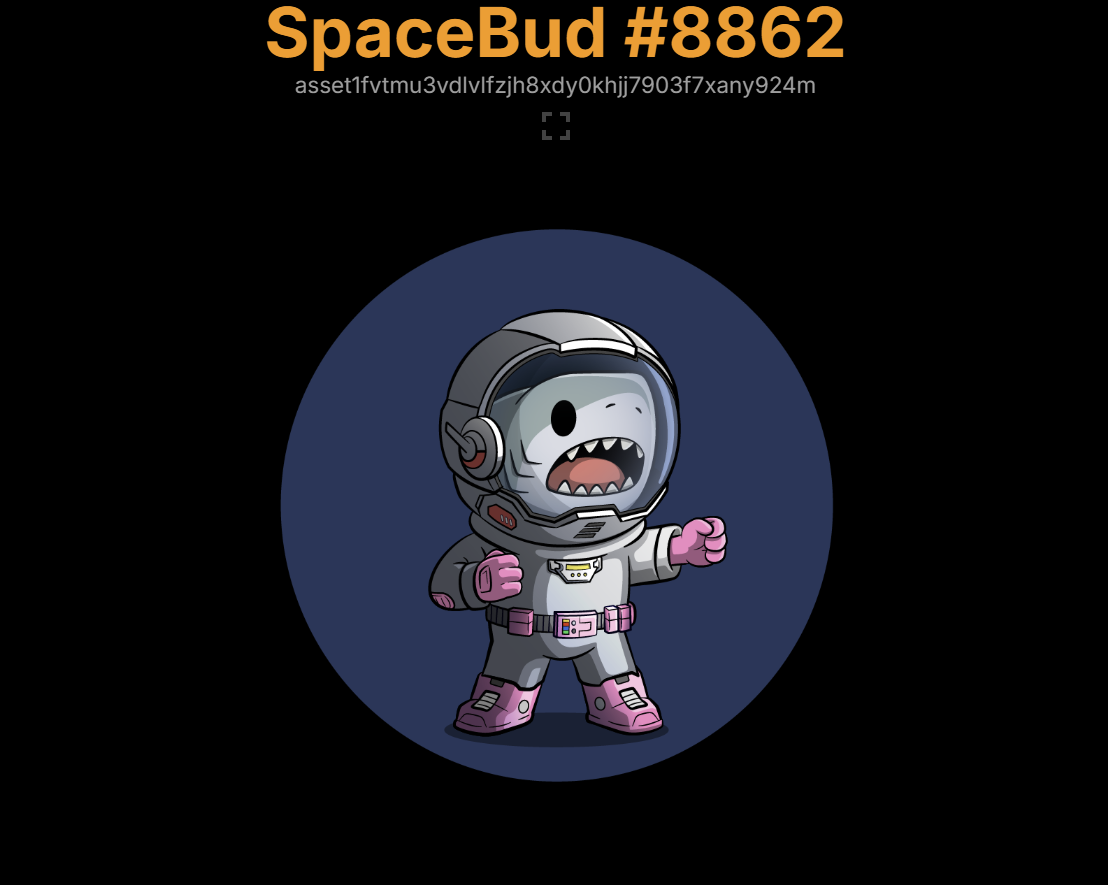
\includegraphics[width=0.35\textwidth]{images/spacebud.png}
    \caption{The SpaceBud NFT used as the governance token for this DRep smart contract}
    \label{fig:spacebud-nft}
\end{figure}

\subsubsection{Why Sign with the Stake Key?}

An important design choice in this contract is that it verifies the \textbf{stake credential} of the address holding the NFT, rather than the spending credential. This is deliberate and enables a powerful delegation pattern:

A Cardano address is composed of two parts -- a \textbf{payment (spending) key} and a \textbf{stake key}. These can belong to different parties. By checking the stake key, the NFT owner can place the NFT at an address where:
\begin{itemize}
    \item The \textbf{spending key} remains under their control, so they never lose custody of the NFT.
    \item The \textbf{stake key} belongs to someone else, effectively delegating governance authority to that person.
\end{itemize}

This means the NFT owner can delegate DRep voting power to a trusted party without ever transferring the NFT itself. If they want to revoke the delegation, they simply move the NFT to an address with a different stake key. This is a clean separation of asset ownership from governance authority, made possible by Cardano's dual-key address model.

\begin{figure}[ht]
    \centering
    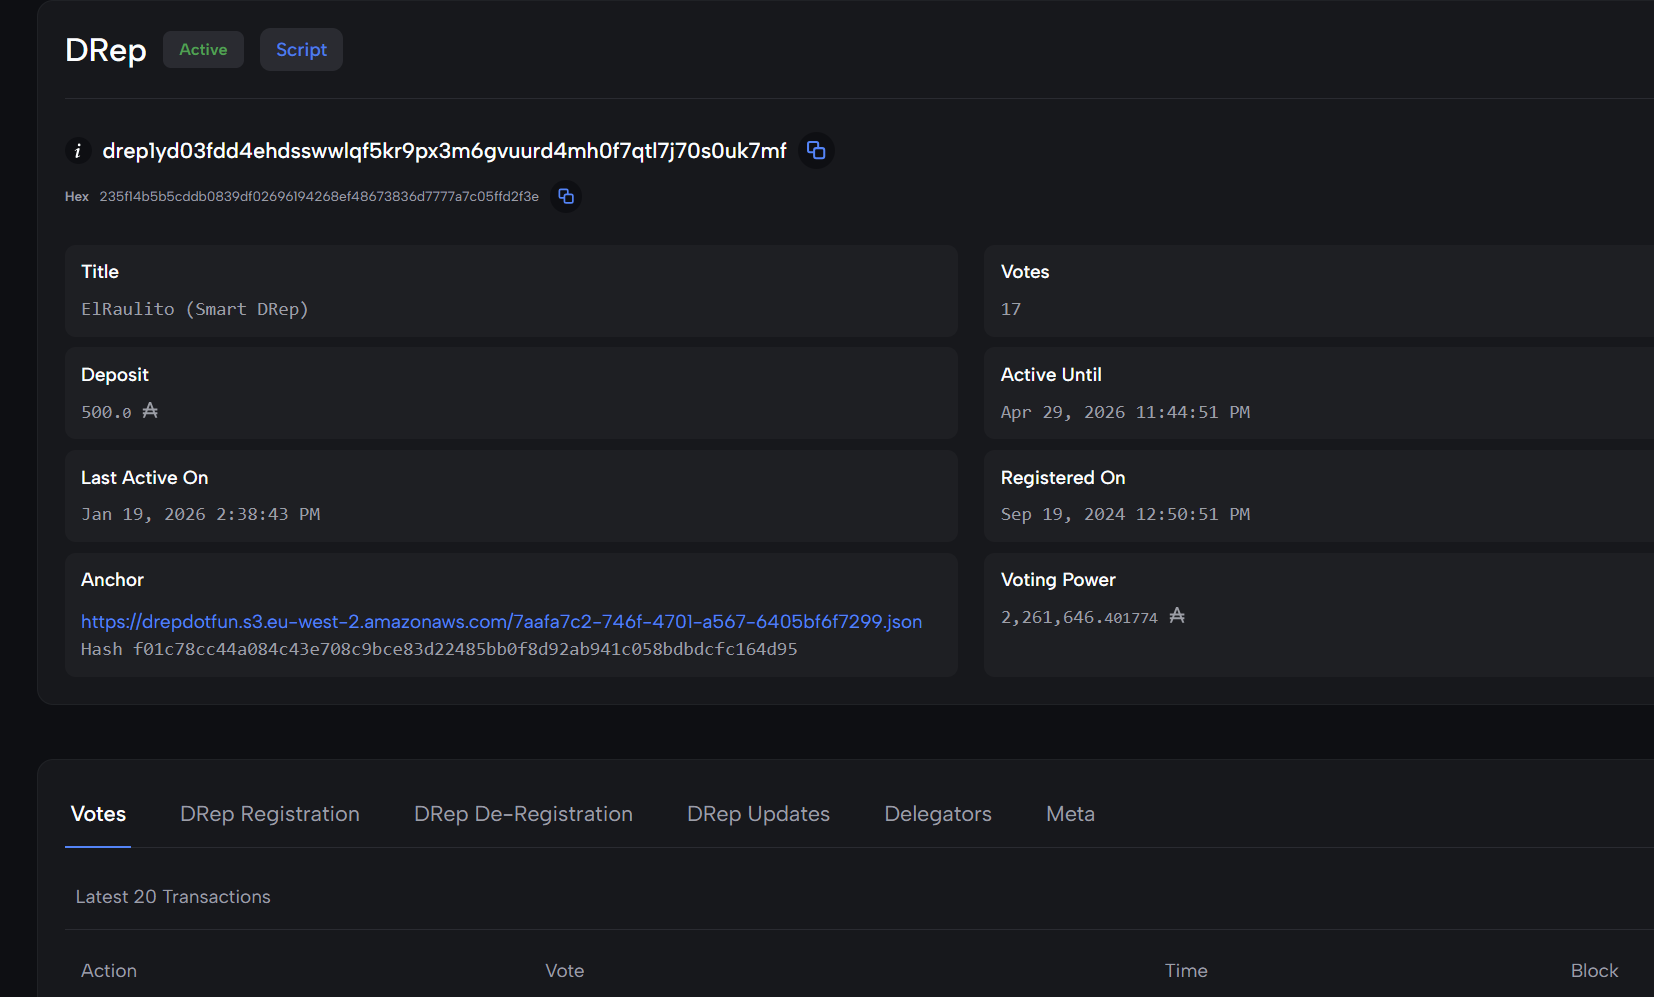
\includegraphics[width=0.8\textwidth]{images/Drep_smartcontract_deployed.png}
    \caption{A deployed DRep smart contract on Cardano mainnet}
    \label{fig:drep-deployed}
\end{figure}

\subsection{Governance Transactions with MeshJS}

MeshJS provides a comprehensive API for building governance transactions in TypeScript/JavaScript. This section demonstrates the key governance operations.

\subsubsection{Setting Up the Transaction Builder}

All governance transactions follow a similar pattern using the \texttt{MeshTxBuilder}:

\begin{lstlisting}[caption=MeshJS Transaction Builder Setup]
import { MeshTxBuilder, BlockfrostProvider }
  from "@meshsdk/core";

const provider =
  new BlockfrostProvider("<YOUR_API_KEY>");
const txBuilder = new MeshTxBuilder({
  fetcher: provider,
  verbose: true,
});
\end{lstlisting}

\subsubsection{Delegating Voting Power to a DRep}

Ada holders can delegate their voting power to a registered DRep using the \texttt{voteDelegationCertificate} method:

\begin{lstlisting}[caption=Delegating Voting Power to a DRep]
const utxos = await wallet.getUtxos();
const changeAddress = await wallet.getChangeAddress();
const rewardAddresses =
  await wallet.getRewardAddresses();
const rewardAddress = rewardAddresses[0];

const dRepId =
  "drep1yv4uesaj92wk8ljlsh4p7jzndnzrflchaz5fzug3zxg4naqkpeas3";

txBuilder
  .voteDelegationCertificate({ dRepId }, rewardAddress)
  .changeAddress(changeAddress)
  .selectUtxosFrom(utxos);

const unsignedTx = await txBuilder.complete();
const signedTx = await wallet.signTx(unsignedTx);
const txHash = await wallet.submitTx(signedTx);
\end{lstlisting}

The \texttt{DRepId} object supports three delegation modes:
\begin{itemize}
    \item \texttt{\{ dRepId: "drep1..." \}} -- Delegate to a specific DRep
    \item \texttt{\{ alwaysAbstain: true \}} -- Always abstain from voting
    \item \texttt{\{ alwaysNoConfidence: true \}} -- Always vote no confidence
\end{itemize}

\subsubsection{Registering as a DRep}

To register as a DRep, you need to provide metadata following the CIP-119 standard:

\begin{lstlisting}[caption=Registering as a DRep with Metadata]
import { MeshTxBuilder, BlockfrostProvider,
  hashDrepAnchor } from "@meshsdk/core";

const dRep = await wallet.getDRep();
const dRepId = dRep.dRepIDCip105;

const anchorUrl =
  "https://example.com/drep-metadata.jsonld";
const anchorMetadata = {
  "@context": {
    "@language": "en",
    "CIP100": "https://github.com/cardano-foundation"
      + "/CIPs/blob/master/CIP-0100/README.md",
    "CIP119": "https://github.com/cardano-foundation"
      + "/CIPs/blob/master/CIP-0119/README.md",
    "hashAlgorithm": "CIP100:hashAlgorithm",
    "body": { "@id": "CIP119:body" },
    "givenName": "CIP119:givenName"
  },
  "hashAlgorithm": "blake2b-256",
  "body": { "givenName": "My DRep Name" }
};
const anchorHash = hashDrepAnchor(anchorMetadata);

const utxos = await wallet.getUtxos();
const changeAddress = await wallet.getChangeAddress();

txBuilder
  .drepRegistrationCertificate(dRepId, {
    anchorUrl,
    anchorDataHash: anchorHash,
  })
  .changeAddress(changeAddress)
  .selectUtxosFrom(utxos);

const unsignedTx = await txBuilder.complete();
const signedTx = await wallet.signTx(unsignedTx);
const txHash = await wallet.submitTx(signedTx);
\end{lstlisting}

\subsubsection{Voting on Governance Actions}

DReps can cast votes on governance actions using the \texttt{vote} method:

\begin{lstlisting}[caption=Casting a Vote on a Governance Action]
const dRep = await wallet.getDRep();
const dRepId = dRep.dRepIDCip105;
const utxos = await wallet.getUtxos();
const changeAddress = await wallet.getChangeAddress();

const govActionTxHash = "aff2909f8175ee02a8c1bf"
  + "96ff516685d25bf0c6b95aac91f4dfd53a5c0867cc";
const govActionIndex = 0;

txBuilder
  .vote(
    { type: "DRep", drepId: dRepId },
    { txHash: govActionTxHash,
      txIndex: govActionIndex },
    { voteKind: "Yes" }
  )
  .selectUtxosFrom(utxos)
  .changeAddress(changeAddress);

const unsignedTx = await txBuilder.complete();
const signedTx = await wallet.signTx(unsignedTx);
const txHash = await wallet.submitTx(signedTx);
\end{lstlisting}

The \texttt{Voter} object supports three voter types:
\begin{itemize}
    \item \texttt{\{ type: "DRep", drepId: "drep1..." \}} -- DRep voter
    \item \texttt{\{ type: "StakePool", poolId: "pool1..." \}} -- Stake pool operator
    \item \texttt{\{ type: "ConstitutionalCommittee", hotCred: "..." \}} -- Constitutional committee member
\end{itemize}

\subsubsection{Voting with a Plutus Script}

Script-based DReps can vote using Plutus V3 scripts, which enables programmable governance logic:

\begin{lstlisting}[caption=Voting with a Plutus V3 Script]
import { MeshTxBuilder, BlockfrostProvider,
  resolveScriptHash, resolveScriptHashDRepId,
  applyCborEncoding } from "@meshsdk/core";

const utxos = await wallet.getUtxos();
const collateral = await wallet.getCollateral();
const changeAddress = await wallet.getChangeAddress();

const votingScriptCbor =
  applyCborEncoding("your-voting-script-cbor");
const scriptHash =
  resolveScriptHash(votingScriptCbor, "V3");
const scriptDRepId =
  resolveScriptHashDRepId(scriptHash);

txBuilder
  .txIn(
    utxos[0].input.txHash,
    utxos[0].input.outputIndex,
    utxos[0].output.amount,
    utxos[0].output.address
  )
  .txInCollateral(
    collateral[0].input.txHash,
    collateral[0].input.outputIndex,
    collateral[0].output.amount,
    collateral[0].output.address
  )
  .votePlutusScriptV3()
  .vote(
    { type: "DRep", drepId: scriptDRepId },
    { txHash: "abc123...", txIndex: 0 },
    { voteKind: "Yes" }
  )
  .voteScript(votingScriptCbor)
  .voteRedeemerValue("")
  .changeAddress(changeAddress);

const unsignedTx = await txBuilder.complete();
const signedTx = await wallet.signTx(unsignedTx, true);
const txHash = await wallet.submitTx(signedTx);
\end{lstlisting}

\subsubsection{DRep Retirement}

A DRep can retire and reclaim their deposit:

\begin{lstlisting}[caption=Retiring as a DRep]
const dRep = await wallet.getDRep();
const dRepId = dRep.dRepIDCip105;
const utxos = await wallet.getUtxos();
const changeAddress = await wallet.getChangeAddress();

txBuilder
  .drepDeregistrationCertificate(dRepId)
  .selectUtxosFrom(utxos)
  .changeAddress(changeAddress);

const unsignedTx = await txBuilder.complete();
const signedTx = await wallet.signTx(unsignedTx);
const txHash = await wallet.submitTx(signedTx);
\end{lstlisting}


\section{Governance Use Cases and Real-World Examples} \label{sec:governance-use-cases}

\subsection{Building a DRep Delegation Frontend}

One practical use case is building a web frontend that allows ada holders to delegate their voting power to a DRep. The following example demonstrates a Next.js application that connects to a Cardano wallet and submits a vote delegation transaction.

\begin{lstlisting}[caption=DRep Delegation Frontend with Next.js and MeshJS]
import { useEffect, useState } from 'react';
import {
  BrowserWallet, Wallet, MeshTxBuilder,
  MaestroProvider, keepRelevant, Transaction, DRep
} from "@meshsdk/core";

export default function DelegatePage() {
  const [selectedWallet, setSelectedWallet] =
    useState(null);
  const [isConnected, setIsConnected] =
    useState(false);

  const handleConnectWallet = async (walletId) => {
    const wallet =
      await BrowserWallet.enable(walletId, [95]);
    setSelectedWallet(wallet);
    setIsConnected(true);
  };

  const handleVoteDelegation = async (drepId) => {
    if (!selectedWallet) return;

    const maestroProvider = new MaestroProvider({
      network: "Mainnet",
      apiKey: "<YOUR_API_KEY>",
      turboSubmit: false
    });

    const txBuilder = new MeshTxBuilder({
      fetcher: maestroProvider,
      verbose: true
    });

    const changeAddress =
      await selectedWallet.getChangeAddress();
    const utxos = await selectedWallet.getUtxos();
    const rewardAddresses =
      await selectedWallet.getRewardAddresses();
    const rewardAddress = rewardAddresses[0];

    txBuilder
      .selectUtxosFrom(utxos)
      .changeAddress(changeAddress)
      .voteDelegationCertificate(
        { dRepId: drepId }, rewardAddress
      );

    const unsignedTx = await txBuilder.complete();
    const signedTx =
      await selectedWallet.signTx(unsignedTx);
    const txHash =
      await selectedWallet.submitTx(signedTx);

    console.log(`Delegated to DRep: ${txHash}`);
  };

  // ... render wallet selection and delegation UI
}
\end{lstlisting}

This example shows the essential steps:
\begin{enumerate}
    \item Connect to a browser-based Cardano wallet using CIP-30/CIP-95.
    \item Set up a transaction builder with a blockchain provider (Maestro in this case).
    \item Fetch the user's UTxOs, change address, and reward addresses.
    \item Build the vote delegation certificate transaction.
    \item Sign and submit the transaction.
\end{enumerate}

\begin{figure}[ht]
    \centering
    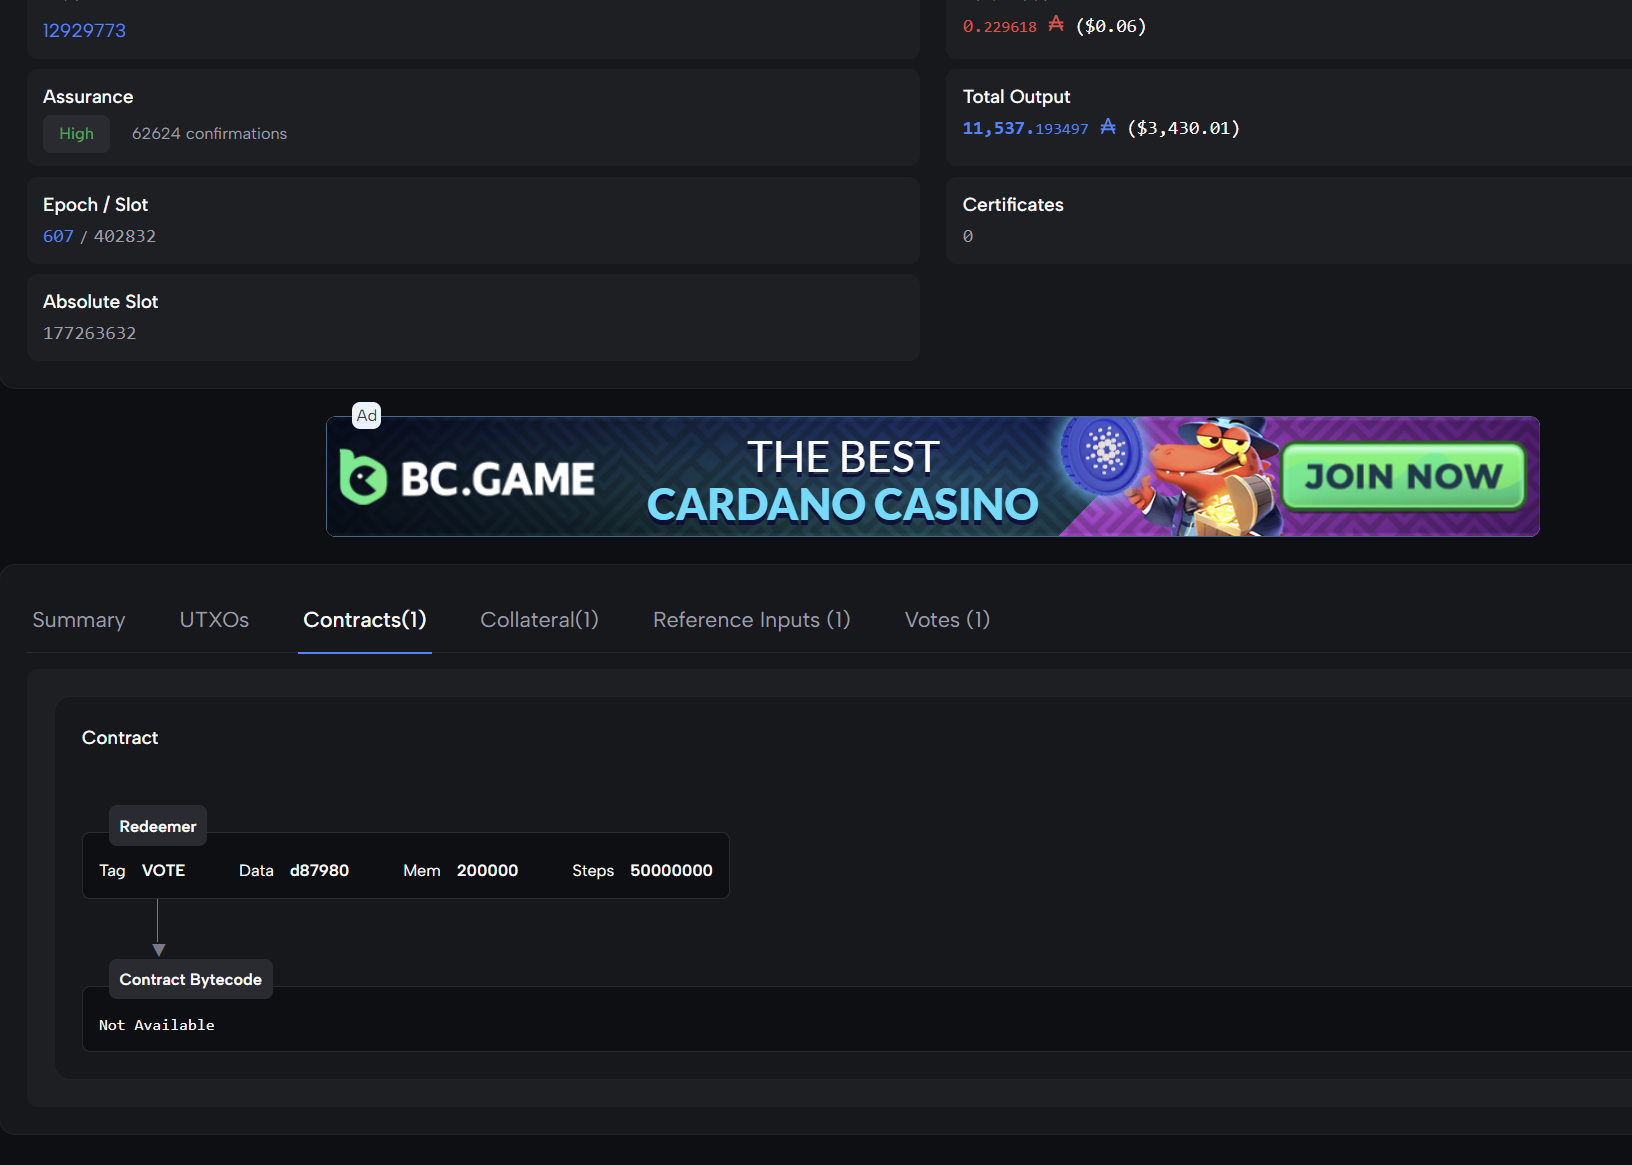
\includegraphics[width=0.8\textwidth]{images/drep_vote.png}
    \caption{A vote executed by a smart contract DRep}
    \label{fig:drep-vote}
\end{figure}

\subsection{Complete DRep Lifecycle}

The following example demonstrates a complete DRep lifecycle, from registration to retirement:

\begin{lstlisting}[caption=Complete DRep Lifecycle Functions]
import { MeshTxBuilder, BlockfrostProvider,
  hashDrepAnchor } from "@meshsdk/core";

const provider =
  new BlockfrostProvider("<YOUR_API_KEY>");

function getTxBuilder() {
  return new MeshTxBuilder({
    fetcher: provider, verbose: true
  });
}

// 1. Register as a DRep
async function registerDRep(wallet, name, url) {
  const txBuilder = getTxBuilder();
  const dRep = await wallet.getDRep();
  const dRepId = dRep.dRepIDCip105;
  const metadata = {
    "@context": { /* CIP-119 context */ },
    "body": { "givenName": name }
  };
  const anchorHash = hashDrepAnchor(metadata);
  const utxos = await wallet.getUtxos();
  const changeAddress =
    await wallet.getChangeAddress();
  txBuilder
    .drepRegistrationCertificate(dRepId, {
      anchorUrl: url,
      anchorDataHash: anchorHash,
    })
    .changeAddress(changeAddress)
    .selectUtxosFrom(utxos);
  const unsignedTx = await txBuilder.complete();
  const signedTx = await wallet.signTx(unsignedTx);
  return await wallet.submitTx(signedTx);
}

// 2. Vote on a governance action
async function castVote(wallet, govActionTxHash,
    govActionIndex, voteKind) {
  const txBuilder = getTxBuilder();
  const dRep = await wallet.getDRep();
  const dRepId = dRep.dRepIDCip105;
  const utxos = await wallet.getUtxos();
  const changeAddress =
    await wallet.getChangeAddress();
  txBuilder
    .vote(
      { type: "DRep", drepId: dRepId },
      { txHash: govActionTxHash,
        txIndex: govActionIndex },
      { voteKind }
    )
    .selectUtxosFrom(utxos)
    .changeAddress(changeAddress);
  const unsignedTx = await txBuilder.complete();
  const signedTx = await wallet.signTx(unsignedTx);
  return await wallet.submitTx(signedTx);
}

// 3. Delegate to a DRep
async function delegateToDRep(wallet, dRepId) {
  const txBuilder = getTxBuilder();
  const utxos = await wallet.getUtxos();
  const changeAddress =
    await wallet.getChangeAddress();
  const rewardAddresses =
    await wallet.getRewardAddresses();
  const rewardAddress = rewardAddresses[0];
  txBuilder
    .voteDelegationCertificate(
      { dRepId }, rewardAddress)
    .changeAddress(changeAddress)
    .selectUtxosFrom(utxos);
  const unsignedTx = await txBuilder.complete();
  const signedTx = await wallet.signTx(unsignedTx);
  return await wallet.submitTx(signedTx);
}

// 4. Retire as DRep
async function retireDRep(wallet) {
  const txBuilder = getTxBuilder();
  const dRep = await wallet.getDRep();
  const dRepId = dRep.dRepIDCip105;
  const utxos = await wallet.getUtxos();
  const changeAddress =
    await wallet.getChangeAddress();
  txBuilder
    .drepDeregistrationCertificate(dRepId)
    .selectUtxosFrom(utxos)
    .changeAddress(changeAddress);
  const unsignedTx = await txBuilder.complete();
  const signedTx = await wallet.signTx(unsignedTx);
  return await wallet.submitTx(signedTx);
}
\end{lstlisting}

\subsection{Lessons from Other Ecosystems: The Polkadot Treasury Case}

Cardano is not the only blockchain with on-chain governance. Polkadot implemented its own model (OpenGov), which includes delegated voting and on-chain treasury management. However, Polkadot's experience serves as a \textbf{cautionary tale} rather than a model to follow.

\begin{figure}[ht]
    \centering
    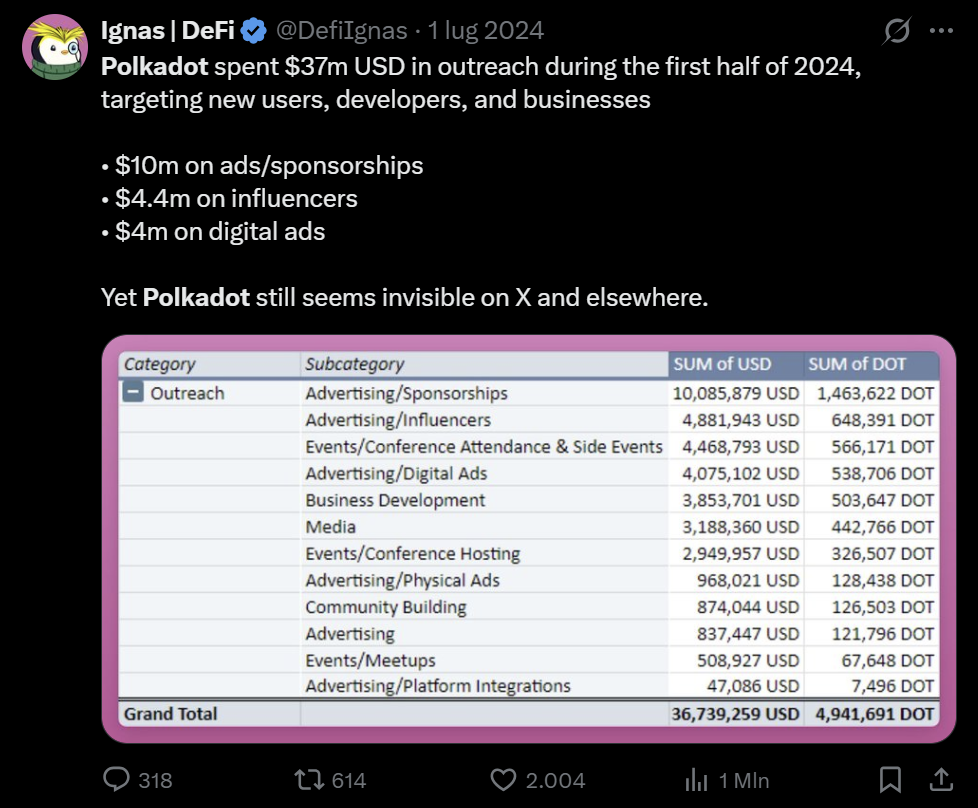
\includegraphics[width=0.8\textwidth]{images/Examples_onchain_polkadot_governance.png}
    \caption{On-chain governance proposals in the Polkadot ecosystem}
    \label{fig:polkadot-governance}
\end{figure}

Polkadot's treasury was effectively drained through governance proposals that delivered little measurable impact on the ecosystem. Large sums were approved for marketing campaigns, events, and initiatives that failed to produce meaningful results in terms of adoption, developer growth, or ecosystem value. The lack of rigorous accountability mechanisms and the low barrier for approval meant that funds flowed out faster than they could generate returns for the network.

This outcome highlights a fundamental challenge of on-chain treasury governance: \textbf{the ability to vote on spending is meaningless without the discipline to vote responsibly.} A governance system is only as good as the quality of decisions made by its participants.

\subsection{Cardano Treasury: A Responsibility, Not Just a Feature}

The Cardano treasury is a pool of ada accumulated from transaction fees and monetary expansion. It is governed by the community through governance actions of type \texttt{TreasuryWdrl}. Treasury withdrawals require approval from both DReps and the Constitutional Committee.

\begin{figure}[ht]
    \centering
    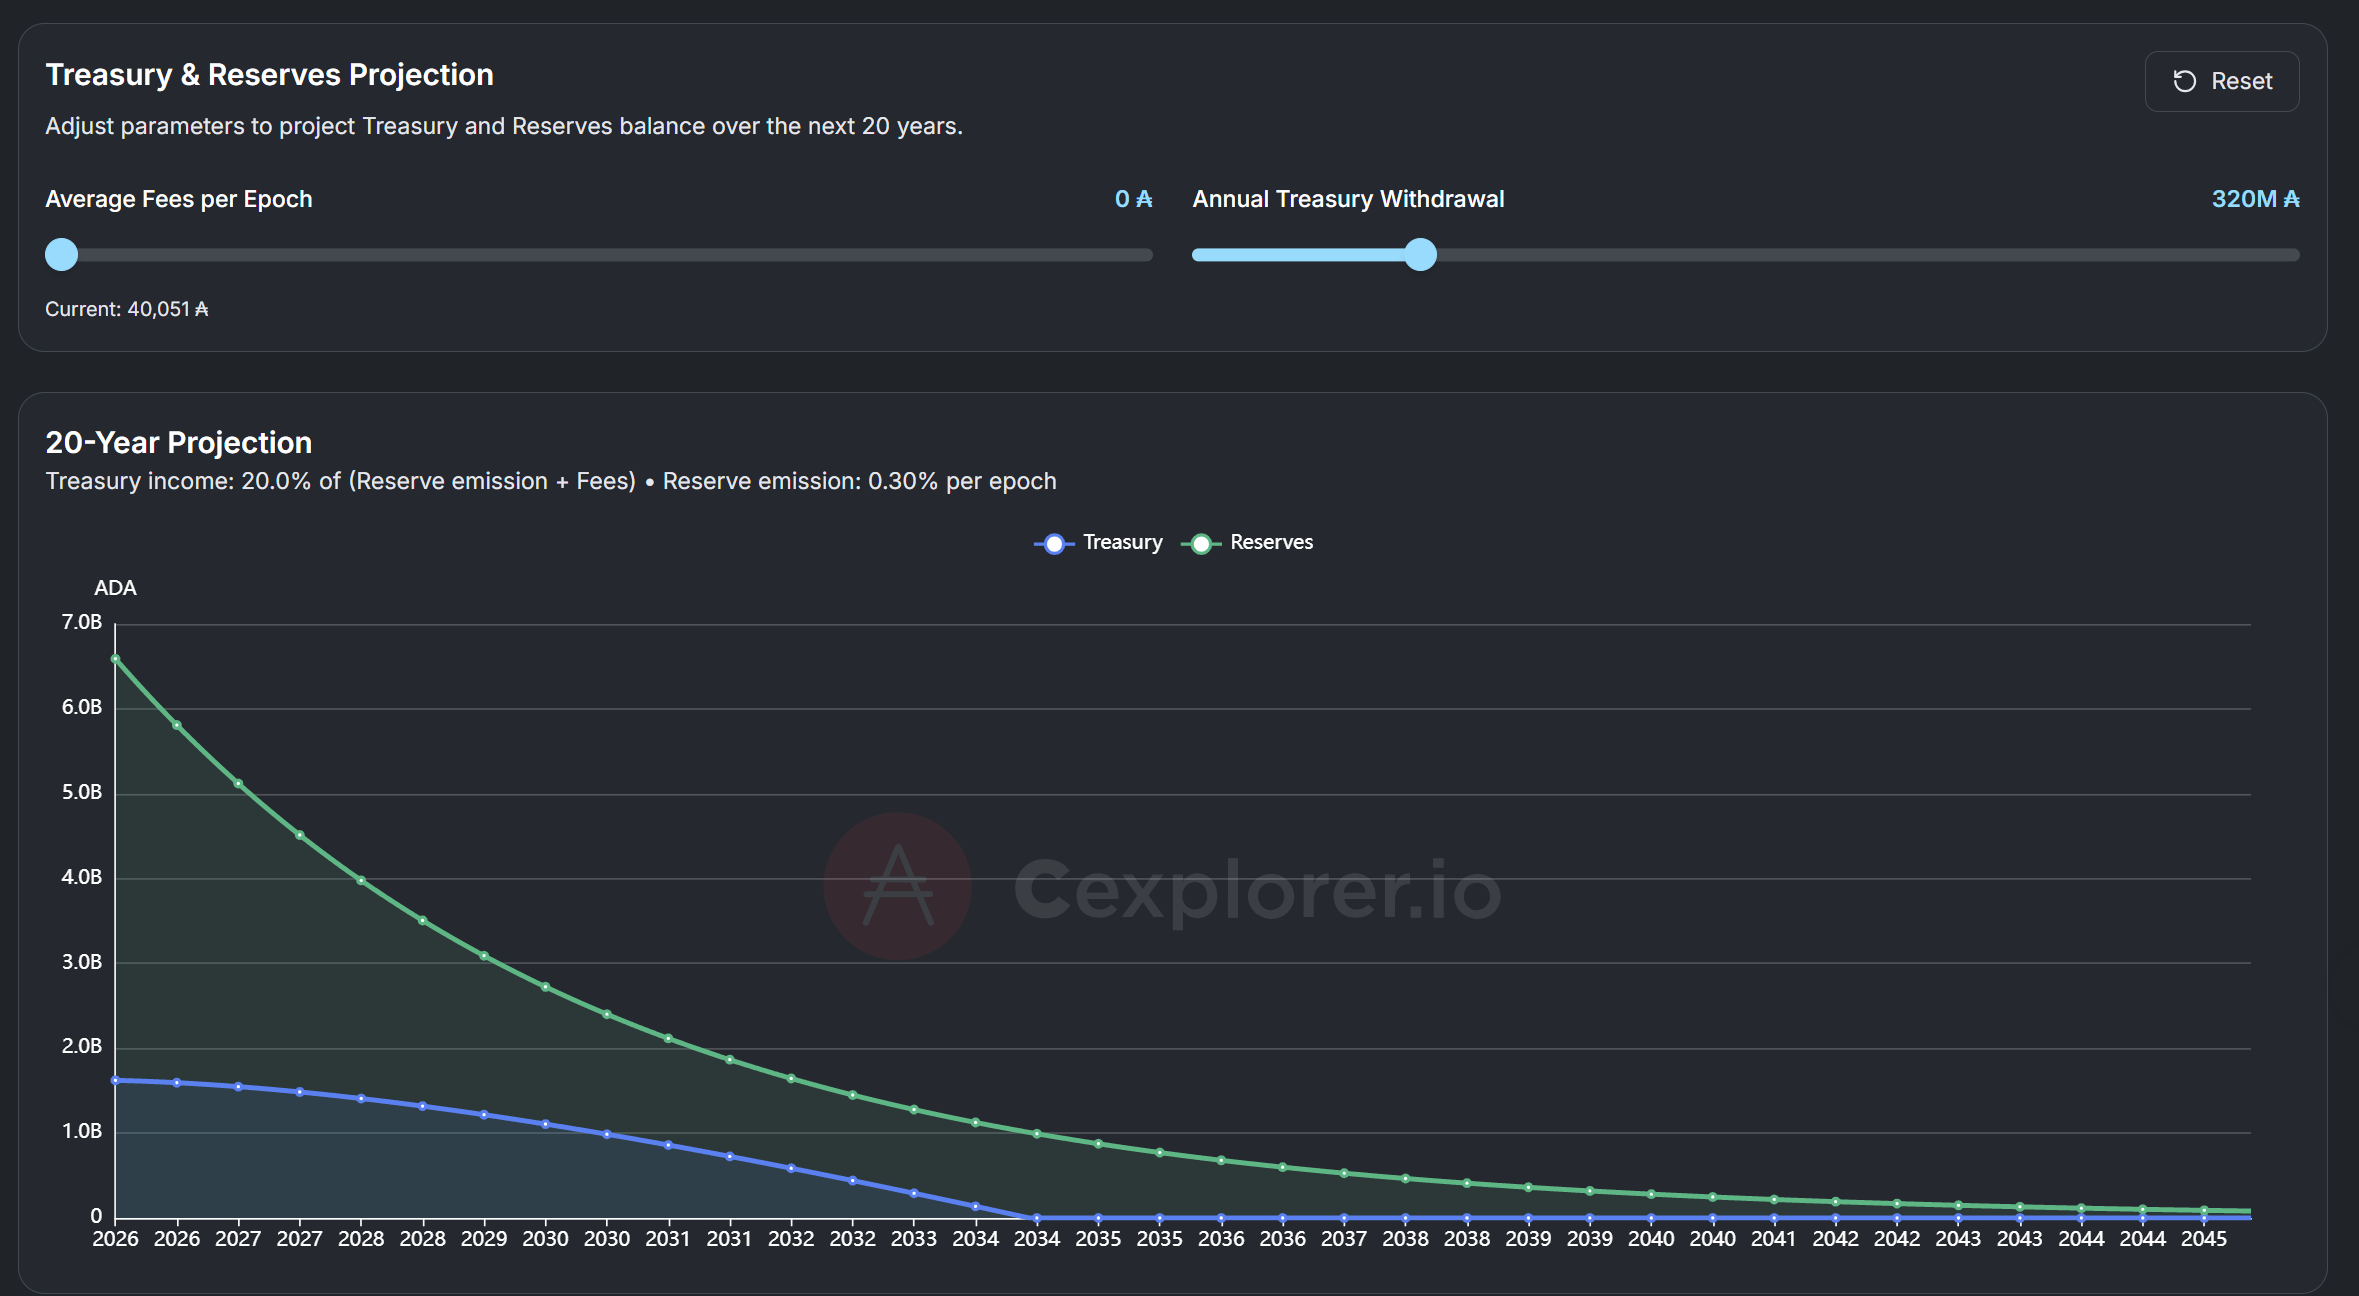
\includegraphics[width=0.8\textwidth]{images/Cexplorer_treaserury_projection_Cardano.png}
    \caption{Cardano treasury projection from Cexplorer}
    \label{fig:treasury-projection}
\end{figure}

Before approving treasury withdrawals, DReps must approve a net change limit and budget through Info actions. This ensures that treasury funds are managed responsibly and in accordance with the Cardano Constitution.

Learning from the mistakes of other ecosystems, Cardano's governance participants -- DReps, SPOs, and the Constitutional Committee -- must exercise careful judgment when voting on treasury withdrawals. Key principles to keep in mind:

\begin{itemize}
    \item \textbf{Demand accountability:} Every treasury proposal should include clear deliverables, timelines, and measurable success criteria.
    \item \textbf{Evaluate impact:} Proposals should demonstrate how they will contribute to the long-term growth and sustainability of the Cardano ecosystem.
    \item \textbf{Protect the treasury:} The treasury is a finite resource. Voting ``Yes'' on every proposal is not participation -- it is negligence.
    \item \textbf{Follow the Constitution:} The Cardano Constitution provides guardrails for treasury management. DReps should familiarize themselves with Article IV, which governs treasury operations.
\end{itemize}

The strength of Cardano's governance will ultimately be measured not by the sophistication of its mechanisms, but by the quality of the decisions its community makes.

\subsection{Common Issues and Troubleshooting}

When working with governance transactions, you may encounter the following common issues:

\begin{itemize}
    \item \textbf{``DRep not registered'' error:} You must register as a DRep before voting. Use \texttt{drepRegistrationCertificate()} first.
    \item \textbf{``Invalid anchor hash'' error:} The hash must match the content at the URL exactly. Use \texttt{hashDrepAnchor()} to compute the correct hash and ensure the metadata file is publicly accessible.
    \item \textbf{``Insufficient deposit'' error:} DRep registration requires a deposit (check current protocol parameters). Ensure the wallet has enough ADA for deposit and fees.
    \item \textbf{``DRep inactive'' error:} DReps must vote regularly to stay active. Vote on governance actions or submit an update certificate.
    \item \textbf{``Governance action not found'' error:} Verify the transaction hash and index are correct. The governance action may have already been resolved.
\end{itemize}

\subsection{Key Takeaways}

\begin{itemize}
    \item Cardano's on-chain governance (CIP-1694) enables decentralized decision-making through three governance bodies: DReps, SPOs, and the Constitutional Committee.
    \item Smart contracts can be used to create programmable DReps, enabling automated or conditional governance participation.
    \item MeshJS provides a comprehensive TypeScript API for building governance transactions including delegation, registration, voting, and retirement.
    \item The governance action lifecycle involves submission, voting within a 6-epoch window, ratification at epoch boundaries, and enactment.
    \item Always test governance transactions on a testnet before deploying to mainnet.
\end{itemize}
